\chapter{Otevřené smlouvy}
\label{sec:kap3}

\section{Situace ve veřejné správě ČR}

Pokud se veřejná instituce rozhodne pro publikaci údajů o smlouvách, má dnes (rok 2015) v podstatě dvě možnosti. První možností je vyvinutí vlastní iniciativy a zveřejnění smluv na svých webových stránkách. Druhou variantou je využití již existujícího registru smluv na portálu veřejné správy\cite{portalgov}. Registr je to značně minimalistický, ale řešení je to dostačující.

Vzhledem k chystanému zákonu o registru smluv se ale budoucnost stávajícího registru jeví jako značně nejistá. Lze totiž očekávat, že s velkou pravděpodobností vznikne registr zbrusu nový\footnote{Zákon o Registru smluv - tisk 42\cite{z42} byl definitivně schválen 24.11.2015 poslaneckou sněmovnou. Neprošel však ještě celým legislativním procesem. Je už ale téměř jisté, že opravdu vznikne nový registr smluv.}.

První otázkou je, kolik veřejných institucí již smlouvy zveřejňuje. Na portálu veřejné správy lze dohledat řádově několik desítek subjektů. O těchto institucích můžeme prohlásit, že oficiálně zveřejňují smlouvy. Informace o subjektech, které zveřejňují na svých webových stránkách, není systematicky zdokumentovaná vůbec. Lze ale očekávat, vzhledem k celkovému množství veřejných institucí a počtu subjetků zveřejňujících na portálu veřejné správy, že se jedná o nepatrný zlomek. Klíčem ke zlepšení situace by mohl být již zmíněný zákon o registru smluv, který mimo jiné ukládá povinnost, že pokud smlouva není zveřejněná na internetu, tak je neplatná.

Další otázkou je, jak mají data o zveřejněných smlouvách vypadat, které položky musí, či nemusí obsahovat. Není přeci cílem, aby každá veřejná instituce zveřejňovala smlouvy jinak. Obecně chybí datový standard a metodika pro zveřejňování smluv. Pokrok v tomto směru udělalo Ministerstvo vnitra ČR, které plánuje vydat sadu standardů pro publikovatelné datové sady veřejných institucí\footnote{Standardy publikace a katalogizace otevřených dat veřejné správy ČR\cite{odgov}}. Bude se mimo jiné jednat o jakési minimální nutné doporučení, co konkrétní datová sada musí obsahovat.

V úvodu již bylo řečeno, že pod záštitou Oživení o.s.\cite{oz} a EconLabu\cite{econLab} (dříve Centrum aplikované ekonomie o.s.) vzniká datový standard pro otevřené smlouvy. Hlavními postavami koordinujícími vývoj standardu se stali PhDr. Ing. Jiří Skuhrovec a Mgr. Lenka Franková. Na tvorbě standardu participuji a mohu konstatovat, že základní verze je již hotová\footnote{Původní, nerozšířený koncept standardu vyplynuvší z práce akční skupiny je k nalezení na webu iniciativy Bezkorupce\cite{standard}}. Velmi pozitivní zprávou je to, že se tento standard s velkou pravděpodobností dostane do oficiálního doporučení Ministerstva vnitra ČR. Zdá se tedy, že celá tato snaha má smysl.

Standardem pro smlouvy to ale nekončí. Myšlenka úzké spolupráce zástupců měst a obcí, akademické a neziskové sféry se osvědčila. Výsledkem je vznik organizace Otevřená města\cite{otv}, která má za cíl sdružovat veřejné instituce. Pod společnou taktovkou pak financovat společné otevřené projekty. Prvním společným projektem je právě registr smluv.

\section{Standard pro zveřejňování smluv}

V této kapitole se podrobněji seznámíme se standardem pro zveřejňování smluv. Nejdříve je vyložena základní struktura datového standardu, poté jsou popsány konkrétní položky standardu a číselníky. Následně jsou popsány způsoby publikace. Na závěr zmíníme několik informací o vznikající metodice pro zveřejňování smluv. 

\subsection{Základní struktura}

Základním objektem, který slouží k reprezentaci dat, je dokument. Jedná se o abstraktní entitu, která nabývá tří rozšíření typu smlouva/příloha/dodatek. Tato rozšíření obsahují všechny položky obsažené v dokumentu a navíc konkrétní položky pro daný typ.
Smluvní strany jsou separátní objekty navázané buď na smlouvu, objednávku nebo fakturu pomocí jednoznačného identifikátoru.
Objednávka a faktura jsou separátní objekty, které se mohou vázat na konkrétní smlouvu/přílohu/dodatek pomocí jednoznačného identifikátoru.
Rozšiřující entity mohou být součástí smlouvy, příp. objednávky. Reprezentují důležité události v životním cyklu dokumentu a jednotlivé transakce (viz. Obr. \ref{obr:standardDatamodel}). 

\begin{figure}[H]
\centerline{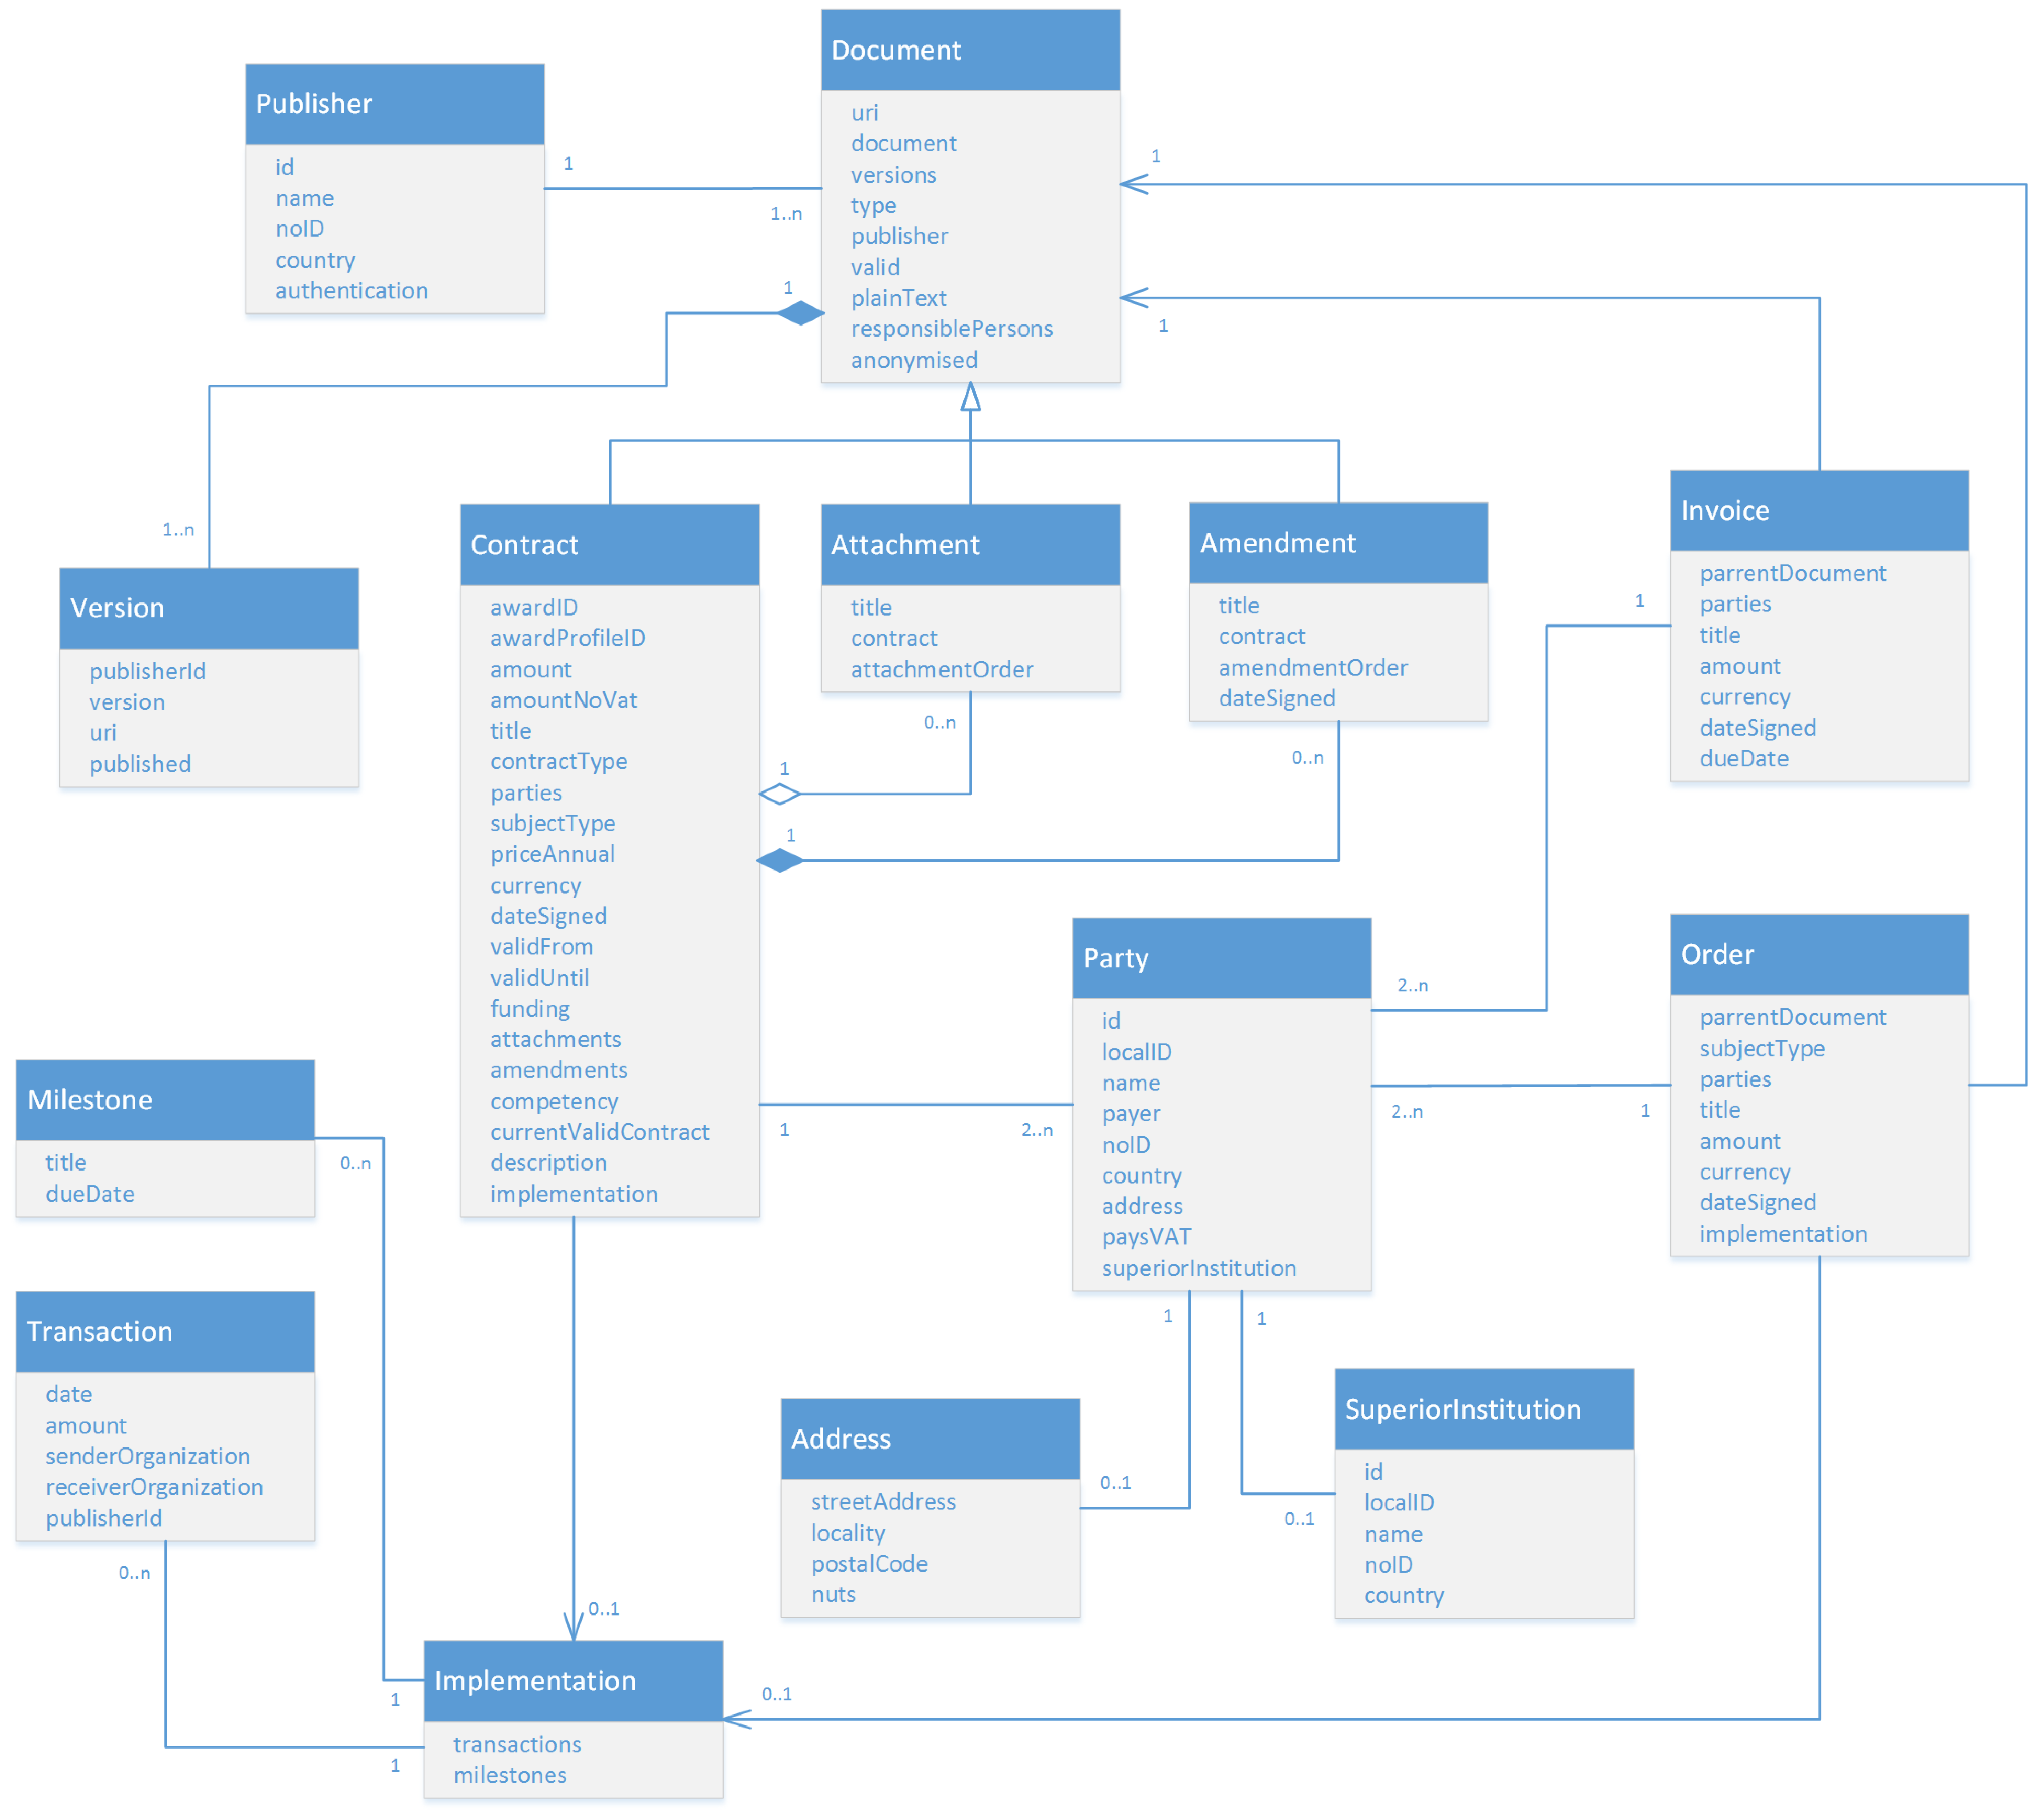
\includegraphics[width=\textwidth]{img/standardDatamodel.eps}}
\caption{Datový standard pro zveřejňování smluv - UML diagram}
\label{obr:standardDatamodel}
\end{figure}

\subsubsection*{Reprezentované entity}

\begin{itemize}
\item \textbf{Dokument} - základní abstraktní struktura pro evidování údajů o smlouvách/přílohách/dodatcích
	\begin{itemize}
    \item \textbf{Smlouva} - detailní popisné údaje smlouvy
    \item \textbf{Příloha} - popisné údaje přílohy 
    \item \textbf{Dodatek} - popisné údaje dodatku
    \item \textbf{Vydavatel} - informace o vydavateli, který zveřejňuje údaje o smlouvách
    \item \textbf{Verze} - identifikace jednotlivé verze dokumentu 
	\end{itemize}
\item \textbf{Smluvní strana} - popisné údaje smluvní strany 
	\begin{itemize}
    \item \textbf{Nadřazená instituce} - informace o řídící nebo ovládající právní osobě vystupující u smluvní strany
    \item \textbf{Adresa} - podrobné údaje o adrese u smluvní strany 
	\end{itemize}
\item \textbf{Objednávka} - popisné údaje objednávky, jedná se o doplňující informace k smlouvě/příloze/dodatku
\item \textbf{Faktura} -  popisné údaje faktury, jedná se o doplňující informace k smlouvě/příloze/dodatku
\item \textbf{Rozšiřující entity} - rozšířené informace ke smlouvě, příp. objednávce
	\begin{itemize}
    \item \textbf{Milník} - reprezentuje důležitou událost v životním cyklu smlouvy
    \item \textbf{Transakce } - reprezentuje proběhlou platbu na základě smlouvy 
	\end{itemize}
\end{itemize}

Datový model je rozdělen do tabulek podle jednotlivých reprezentovaných entit. Každá dílčí položka entity obsahuje tyto informace:

\begin{table}[h]
\centering
\rowcolors{1}{validateB}{validateB}
\begin{tabular}{ll}
\hiderowcolors \textbf{Název pole} & \textbf{Popis} \\ \showrowcolors
\hline
Název pole & Jméno reprezentující danou položku \\
Datový typ & Přípustný datový typ položky \\
Validita & Stupeň kvality položky. \\
Popis & Podrobný popis položky \\
\end{tabular}
\caption{Položky tabulek datového standardu}
\end{table}

U každé zveřejněné smlouvy rozlišujeme tři stupně validity, resp. správnosti a úplnosti dat: A (kvalitní), B (dobrý), C (základní). Dokumenty musí splňovat alespoň minimální přípustnou kvalitu C. Pokud je nějaký atribut požadován pro stupeň validity C, je níže v textu označen např. takto (C). Položky doplněné systémem jsou označeny (S). Nepovinné položky jsou značeny (N), hvězdička znamená, že položka je kontrolována pokročilejším pravidlem popsaném u konkrétní položky. 

\begin{table}[h]
\centering
\begin{tabular}{lcl}
\textbf{Status} & \textbf{Validita} & \textbf{Popis} \\
\hline
Nepovinné & N & Nepovinná položka \\
\rowcolor{validateC}Základní & C & Povinná položka \\
\rowcolor{validateB}Dobrý & B & Rozšiřující položka pro status \uv{Dobrý} \\
\rowcolor{validateA}Kvalitní & A & Rozšiřující položka pro status \uv{Kvalitní} \\
\rowcolor{validateS}Systémové & S & Položka doplněná systémem \\
\end{tabular}
\caption{Validita}
\end{table}

\subsubsection*{Doplňující validační pravidla}

Na entity se vztahují další validační pravidla, která nelze přehledně zachytit v rámci popisu jednotlivých položek. Jejich výčet je zde.

\begin{itemize}
\item Dokument je buď v strojově čitelném formátu (viz. Akceptovatelné soubory), nebo je k němu poskytnut plain text. Pro smlouvy účinné od 1.6.2015\footnote{Předběžné, bude upřesněno} je přípustná pouze varianta ve strojově čitelném formátu.
\item U smlouvy typu darovací nesmí být připojeny faktury, ani jedna smluvní strana nesmí být identifikována jako Payer.
\item Entita (Vydavatel/Smluvní strana/Nadřazená instituce) má vyplněno buď ID, a nebo NoID = \uv{true}.
\end{itemize}

\subsubsection*{Akceptovatelné soubory}

Dokumenty připojené ke smlouvám by měly být strojově čitelné, resp. v těchto formátech:

\begin{table}[h]
\centering
\begin{tabular}{lcl}
\textbf{Formát} & \textbf{Validita} & \textbf{Popis} \\
\hline
\rowcolor{validateC}PDF & C & Portable Document Format - ideálně strojově čitelný \\
\rowcolor{validateC}DOC & C & Textový dokument Microsoft Word \\
\rowcolor{validateC}XLS & C & Tabulka Microsoft Excel \\
\rowcolor{validateB}DOCX & B & Textový dokument Microsoft Word \\
\rowcolor{validateB}ODT & B & Textový dokument OpenDocument \\
\rowcolor{validateB}XLSX & B & Tabulka Microsoft Excel \\
\rowcolor{validateB}ODS & B & Tabulka OpenDocument \\
\end{tabular}
\caption{Akceptovatelné soubory}
\end{table}

\newpage

\subsection{Reprezentované entity}

\medskip

\subsubsection*{Dokument}

\begin{center}
\begin{longtable}{lp{20mm}cp{65mm}}
\label{grid_mlmmh} \\
\multicolumn{1}{l}{\textbf{Název pole}} & 
\multicolumn{1}{l}{\textbf{Datový typ}} & 
\multicolumn{1}{l}{\textbf{Validita}} & 
\multicolumn{1}{l}{\textbf{Popis}} \\ \hline 
\endfirsthead
\multicolumn{1}{l}{\textbf{Název pole}} & 
\multicolumn{1}{l}{\textbf{Datový typ}} & 
\multicolumn{1}{l}{\textbf{Validita}} & 
\multicolumn{1}{l}{\textbf{Popis}} \\ \hline 
\hline
\endhead
\endfoot
\caption{Vlastnosti dokumentu}
\endlastfoot
\rowcolor{validateS}URI & String URI & S & Jednoznačný identifikátor formou URL. Typicky rsmluv.cz/[Typ]/[Id]/[Version], kde Version je vzestupné číslování verzí při změnách dokumentu či metadat \\
\rowcolor{validateS}Document & String URI & S & Adresa URL fyzického umístění dokumentu. Typicky rsmluv.cz/[Typ]/[Id]/[Version]/File, viz akceptovatelné soubory \\
\rowcolor{validateS}Versions & Object array & S & Údaje o verzi dokumentu. Viz entitia Verze \\
\rowcolor{validateC}Type & String/ String enum & C & Typ dokumentu. Nabývá hodnot - Smlouva/Příloha/Dodatek \\
\rowcolor{validateC}Publisher & Reference & C & Informace o vydavateli. Viz entitia Vydavatel \\
\rowcolor{validateB}Valid & Boolean & B/S & Indikuje, zda dokument je platný, tj. nebyl zneplatněn nebo nahrazen novou verzí \\
\rowcolor{validateB}PlainText & String & B/S & Prostý text dokumentu (nestrukturovaný, indexovatelný), alternativa pro scanované dokumenty \\
\rowcolor{validateB}ResponsiblePersons & String array & B & Výčet odpovědných osob \\
\rowcolor{validateB}Anonymised & Boolean & B & Značí, zda-li byla provedena anonymizace dokumentu \\
\end{longtable}
\end{center}

\subsubsection*{Vydavatel}

\begin{center}
\begin{longtable}{lp{20mm}cp{65mm}}
\label{grid_mlmmh} \\
\multicolumn{1}{l}{\textbf{Název pole}} & 
\multicolumn{1}{l}{\textbf{Datový typ}} & 
\multicolumn{1}{l}{\textbf{Validita}} & 
\multicolumn{1}{l}{\textbf{Popis}} \\ \hline 
\endfirsthead
\multicolumn{1}{l}{\textbf{Název pole}} & 
\multicolumn{1}{l}{\textbf{Datový typ}} & 
\multicolumn{1}{l}{\textbf{Validita}} & 
\multicolumn{1}{l}{\textbf{Popis}} \\ \hline 
\hline
\endhead
\endfoot
\caption{Vlastnosti vydavatele}
\endlastfoot
ID & String & N & Identifikační číslo osoby, lze vložit i zahraniční ID \\
\rowcolor{validateC}Name & String & C & Název, případně jméno a příjmení (s tituly) \\
\rowcolor{validateB}NoID & Boolean & B & Indikuje že subjekt nemá IČ, nebo zahraniční ID \\
\rowcolor{validateB}Country & String & B & Země původu, 3-písmený ISO kód \\
\rowcolor{validateS}Authentication & String & S & Značí stupeň ověřenosti zveřejňující strany \\
\end{longtable}
\end{center}

\newpage

\subsubsection*{Verze}

\begin{center}
\begin{longtable}{lp{20mm}cp{65mm}}
\label{grid_mlmmh} \\
\multicolumn{1}{l}{\textbf{Název pole}} & 
\multicolumn{1}{l}{\textbf{Datový typ}} & 
\multicolumn{1}{l}{\textbf{Validita}} & 
\multicolumn{1}{l}{\textbf{Popis}} \\ \hline 
\endfirsthead
\multicolumn{1}{l}{\textbf{Název pole}} & 
\multicolumn{1}{l}{\textbf{Datový typ}} & 
\multicolumn{1}{l}{\textbf{Validita}} & 
\multicolumn{1}{l}{\textbf{Popis}} \\ \hline 
\hline
\endhead
\endfoot
\caption{Vlastnosti verze smlouvy}
\endlastfoot
PublisherId & String & N & Libovolný číselný identifikátor verze, spisové číslo apod. \\
\rowcolor{validateS}Version & Int & S & Pořadové číslo verze, nejvyšší = aktuální \\
\rowcolor{validateS}URI & String URI & S & Identifikátor dané verze \\
\rowcolor{validateS}Published & DateTime & S & Datum publikace v systému \\
\end{longtable}
\end{center}

\subsubsection*{Smlouva}

\begin{center}
\begin{longtable}{lp{20mm}cp{65mm}}
\label{grid_mlmmh} \\
\multicolumn{1}{l}{\textbf{Název pole}} & 
\multicolumn{1}{l}{\textbf{Datový typ}} & 
\multicolumn{1}{l}{\textbf{Validita}} & 
\multicolumn{1}{l}{\textbf{Popis}} \\ \hline 
\endfirsthead
\multicolumn{1}{l}{\textbf{Název pole}} & 
\multicolumn{1}{l}{\textbf{Datový typ}} & 
\multicolumn{1}{l}{\textbf{Validita}} & 
\multicolumn{1}{l}{\textbf{Popis}} \\ \hline 
\hline
\endhead
\endfoot
\caption{Vlastnosti smlouvy}
\endlastfoot
AwardID & String & N* & Evidenční číslo veřejné zakázky. Uvádí se volitelně, pokud existuje \\
AwardProfileID & String & N & Číslo zakázky na profilu zadavatele \\
\rowcolor{validateC}Amount\footnote{U položek Amount a AmountNoVat připustíme místo ceny vyplněný objekt složený z položek AmountValue (cena) a Currency (měna). Je to z důvodu lepšího zapouzdření informací o ceně.} & Nullable float & C* & Cena s DPH (u neplátců celková cena). Nejvyšší přípustná hodnota řádného plnění z dané smlouvy, které vynaloží některá smluvní strana. U smluv na dobu určitou se jedná o očekávané celkové finanční plnění strany s nejvyšším plněním, včetně opcí, bez sankcí. U smluv na dobu neurčitou, ve kterých není stanoven strop na celkové plnění, se jedná o nejvyšší očekávané roční plnění. U smluv bez finančního plnění (bartery, darovací smlouvy) je uvedena celková hodnota nefinančního plnění strany s nejvyšším plněním (např. odhadovaná hodnota daru). U smluv s nejasným plněním připustit NULL. Pokud je cena nenulová, tak alespoň jedna Smluvní strana (Party) musí mít příznak Payer = true \\
\rowcolor{validateC}AmountNoVat & Nullable float & C* & Cena bez dph, uvádí se povinně pouze v případě, že Amount je s DPH \\
\rowcolor{validateC}Title & String & C & Předmět smlouvy \\
\rowcolor{validateC}ContractType & String & C & Číselník typů smlouvy, viz Číselníky \\
\rowcolor{validateC}Parties & StringURI/ Int array & C & Seznam identifikátorů (URI nebo LocalID) smluvních stran. Viz entitia Smluvní strana \\
\rowcolor{validateB}SubjectType & String & B & Číselník typů zboží/služeb, viz. Číselníky \\
\rowcolor{validateB}PriceAnnual & Boolean & B & Identifikuje, pokud je v Amount roční částka \\
\rowcolor{validateB}Currency & String & B & Měna, 3-písmenný, ISO 4217 formát \\
\rowcolor{validateB}DateSigned & Date & B & Datum posledního podpisu \\
\rowcolor{validateB}ValidFrom & Date & B & Datum účinnosti smlouvy \\
\rowcolor{validateB}ValidUntil & Date & B & Datum ukončení účinnosti smlouvy (poslední plnění), NULL pro smlouvy na dobu \\
\rowcolor{validateB}Funding & String & B & Převažující financování – vlastní, případně název dotačního titulu (bude kontrolován proti číselníku, viz. Číselníky) \\
\rowcolor{validateB}Attachments & String URIarray & B & Seznam URI identifikátorů příloh. Viz entitia Příloha \\
\rowcolor{validateB}Amendments & String URIarray & B & Seznam URI identifikátorů dodatků. Viz entitia Dodatek \\
\rowcolor{validateA}Competency & String/ String enum & A & Indikuje, zda-li se jedná o soukromoprávní nebo veřejnoprávní smlouvu \\
\rowcolor{validateA}CurrentValidContract & String URI & A & Aktuálně platné znění smlouvy (se zapracovanými dodatky) \\
\rowcolor{validateA}Description & String & A & Popis předmětu smlouvy \\
\rowcolor{validateA}Implementation & Object & A & Objekt reprezentující transakce a milníky, viz entitia Implementation \\
\end{longtable}
\end{center}

\subsubsection*{Příloha}

\begin{center}
\begin{longtable}{lp{20mm}cp{65mm}}
\label{grid_mlmmh} \\
\multicolumn{1}{l}{\textbf{Název pole}} & 
\multicolumn{1}{l}{\textbf{Datový typ}} & 
\multicolumn{1}{l}{\textbf{Validita}} & 
\multicolumn{1}{l}{\textbf{Popis}} \\ \hline 
\endfirsthead
\multicolumn{1}{l}{\textbf{Název pole}} & 
\multicolumn{1}{l}{\textbf{Datový typ}} & 
\multicolumn{1}{l}{\textbf{Validita}} & 
\multicolumn{1}{l}{\textbf{Popis}} \\ \hline 
\hline
\endhead
\endfoot
\caption{Vlastnosti přílohy}
\endlastfoot
\rowcolor{validateC}Title & String & C & Název \\
\rowcolor{validateC}Contract & String URI & C & Jednoznační identifikátor smlouvy \\
\rowcolor{validateB}AttachmentOrder & Int & B & Pořadové číslo přílohy \\
\end{longtable}
\end{center}

\subsubsection*{Dodatek}

\begin{center}
\begin{longtable}{lp{20mm}cp{65mm}}
\label{grid_mlmmh} \\
\multicolumn{1}{l}{\textbf{Název pole}} & 
\multicolumn{1}{l}{\textbf{Datový typ}} & 
\multicolumn{1}{l}{\textbf{Validita}} & 
\multicolumn{1}{l}{\textbf{Popis}} \\ \hline 
\endfirsthead
\multicolumn{1}{l}{\textbf{Název pole}} & 
\multicolumn{1}{l}{\textbf{Datový typ}} & 
\multicolumn{1}{l}{\textbf{Validita}} & 
\multicolumn{1}{l}{\textbf{Popis}} \\ \hline 
\hline
\endhead
\endfoot
\caption{Vlastnosti dodatku}
\endlastfoot
\rowcolor{validateC}Title & String & C & Název \\
\rowcolor{validateC}Contract & String URI & C & Jednoznační identifikátor smlouvy \\
\rowcolor{validateB}AmendmentOrder & Int & B & Pořadové číslo dodatku (podle času podpisu) \\
\rowcolor{validateB}DateSigned & Date & B & Datum podpisu \\
\end{longtable}
\end{center}

\newpage

\subsubsection*{Smluvní strana}

\begin{center}
\begin{longtable}{lp{20mm}cp{65mm}}
\label{grid_mlmmh} \\
\multicolumn{1}{l}{\textbf{Název pole}} & 
\multicolumn{1}{l}{\textbf{Datový typ}} & 
\multicolumn{1}{l}{\textbf{Validita}} & 
\multicolumn{1}{l}{\textbf{Popis}} \\ \hline 
\endfirsthead
\multicolumn{1}{l}{\textbf{Název pole}} & 
\multicolumn{1}{l}{\textbf{Datový typ}} & 
\multicolumn{1}{l}{\textbf{Validita}} & 
\multicolumn{1}{l}{\textbf{Popis}} \\ \hline 
\hline
\endhead
\endfoot
\caption{Vlastnosti smluvní strany}
\endlastfoot
ID & String & N & Identifikační číslo osoby, lze vložit i zahraniční id \\
\rowcolor{validateC}LocalID & String URI/Int & C & Jednoznačný identifikátor v rámci dokumentu \\
\rowcolor{validateC}Name & String & C & Název, případně jméno a příjmení (s tituly) \\
\rowcolor{validateC}Payer & Boolean & C* & Identifikuje stranu která bude finančně plnit, pokud není zřejmé, nevyplňuje se \\
\rowcolor{validateB}NoID & Boolean & B & Indikuje že subjekt nemá IČ, nebo zahraniční ID \\
\rowcolor{validateB}Country & String & B & Země původu, 3-písmený ISO kód \\
\rowcolor{validateA}Address & String/Reference & A & Adresa subjektu, případně "Anonymizováno". Umožňuje zadat adresu jako prostý řetězec, nebo strukturovaně, viz entitia Adresa \\
\rowcolor{validateA}PaysVAT & Boolean & A & Indikuje, zda-li je subjekt plátce DPH \\
\rowcolor{validateS}SuperiorInstitution & Reference & N/S & Řídící nebo ovládající právnická osoba, v případě  veřejnoprávních smluv nadřízený správní orgán. Viz Nadřazená instituce \\
\end{longtable}
\end{center}

\subsubsection*{Nadřazené instituce}

\begin{center}
\begin{longtable}{lp{20mm}cp{65mm}}
\label{grid_mlmmh} \\
\multicolumn{1}{l}{\textbf{Název pole}} & 
\multicolumn{1}{l}{\textbf{Datový typ}} & 
\multicolumn{1}{l}{\textbf{Validita}} & 
\multicolumn{1}{l}{\textbf{Popis}} \\ \hline 
\endfirsthead
\multicolumn{1}{l}{\textbf{Název pole}} & 
\multicolumn{1}{l}{\textbf{Datový typ}} & 
\multicolumn{1}{l}{\textbf{Validita}} & 
\multicolumn{1}{l}{\textbf{Popis}} \\ \hline 
\hline
\endhead
\endfoot
\caption{Vlastnosti nadřazené instituce}
\endlastfoot
ID & String & N & Identifikační číslo osoby, lze vložit i zahraniční id \\
\rowcolor{validateC}LocalID & String URI/Int & C & Jednoznačný identifikátor v rámci dokumentu \\
\rowcolor{validateC}Name & String & C & Název, případně jméno a příjmení (s tituly) \\
\rowcolor{validateB}NoID & Boolean & B & Indikuje že subjekt nemá IČ, nebo zahraniční ID \\
\rowcolor{validateB}Country & String & B & Země původu, 3-písmený ISO kód \\
\end{longtable}
\end{center}

\newpage

\subsubsection*{Adresa}

\begin{center}
\begin{longtable}{lp{20mm}cp{65mm}}
\label{grid_mlmmh} \\
\multicolumn{1}{l}{\textbf{Název pole}} & 
\multicolumn{1}{l}{\textbf{Datový typ}} & 
\multicolumn{1}{l}{\textbf{Validita}} & 
\multicolumn{1}{l}{\textbf{Popis}} \\ \hline 
\endfirsthead
\multicolumn{1}{l}{\textbf{Název pole}} & 
\multicolumn{1}{l}{\textbf{Datový typ}} & 
\multicolumn{1}{l}{\textbf{Validita}} & 
\multicolumn{1}{l}{\textbf{Popis}} \\ \hline 
\hline
\endhead
\endfoot
\caption{Vlastnosti adresy}
\endlastfoot
\rowcolor{validateA}StreetAddress & String & A & Ulice, případně "Anonymizováno" \\
\rowcolor{validateA}Locality & String & A & Město, případně "Anonymizováno" \\
\rowcolor{validateA}PostalCode & Integer & A & PSČ, případně "Anonymizováno" \\
\rowcolor{validateA}Nuts & String & A & Normalizovaná klasifikace územních celků (např. Praha - CZ010), případně "Anonymizováno" \\
\end{longtable}
\end{center}

\subsubsection*{Objednávka}

\begin{center}
\begin{longtable}{lp{20mm}cp{65mm}}
\label{grid_mlmmh} \\
\multicolumn{1}{l}{\textbf{Název pole}} & 
\multicolumn{1}{l}{\textbf{Datový typ}} & 
\multicolumn{1}{l}{\textbf{Validita}} & 
\multicolumn{1}{l}{\textbf{Popis}} \\ \hline 
\endfirsthead
\multicolumn{1}{l}{\textbf{Název pole}} & 
\multicolumn{1}{l}{\textbf{Datový typ}} & 
\multicolumn{1}{l}{\textbf{Validita}} & 
\multicolumn{1}{l}{\textbf{Popis}} \\ \hline 
\hline
\endhead
\endfoot
\caption{Vlastnosti objednávky}
\endlastfoot
ParrentDocument & String URI & N & Jednoznačný identifikátor dokumentu \\
SubjectType & String & N & Číselník typů zboží/služeb, viz Číselníky \\
Parties & String URI/Int array & N & Seznam identifikátorů (URI nebo LocalID) smluvních stran. Viz entitia Smluvní strana \\
\rowcolor{validateC}Title & String & C & Předmět \\
\rowcolor{validateC}Amount & Float & C & Cena s DPH \\
\rowcolor{validateB}Currency & String & B & Měna, 3-písmenný, ISO 4217 formát \\
\rowcolor{validateB}DateSigned & Date & B & Datum posledního podpisu \\
\rowcolor{validateA}Implementation & Object & A & Objekt reprezentující transakce a milníky, viz entitia Implementation \\
\end{longtable}
\end{center}

\subsubsection*{Faktura}

\begin{center}
\begin{longtable}{lp{20mm}cp{65mm}}
\label{grid_mlmmh} \\
\multicolumn{1}{l}{\textbf{Název pole}} & 
\multicolumn{1}{l}{\textbf{Datový typ}} & 
\multicolumn{1}{l}{\textbf{Validita}} & 
\multicolumn{1}{l}{\textbf{Popis}} \\ \hline 
\endfirsthead
\multicolumn{1}{l}{\textbf{Název pole}} & 
\multicolumn{1}{l}{\textbf{Datový typ}} & 
\multicolumn{1}{l}{\textbf{Validita}} & 
\multicolumn{1}{l}{\textbf{Popis}} \\ \hline 
\hline
\endhead
\endfoot
\caption{Vlastnosti faktury}
\endlastfoot
ParrentDocument & String URI & N & Jednoznačný identifikátor dokumentu \\
Parties & String URI/Int array & N & Seznam identifikátorů (URI nebo LocalID) smluvních stran. Viz entitia Smluvní strana \\
\rowcolor{validateC}Title & String & C & Předmět \\
\rowcolor{validateC}Amount & Float & C* & Cena s DPH (u neplátců celková cena). \\
\rowcolor{validateB}Currency & String & B & Měna, 3-písmenný, ISO 4217 formát \\
\rowcolor{validateB}DateSigned & Date & B & Datum posledního podpisu \\
\rowcolor{validateB}DueDate & Date & B & Datum splatnosti \\
\end{longtable}
\end{center}

\subsubsection*{Rozšiřující entity}

\subsubsection*{Implementace}

\begin{center}
\begin{longtable}{lp{20mm}cp{65mm}}
\label{grid_mlmmh} \\
\multicolumn{1}{l}{\textbf{Název pole}} & 
\multicolumn{1}{l}{\textbf{Datový typ}} & 
\multicolumn{1}{l}{\textbf{Validita}} & 
\multicolumn{1}{l}{\textbf{Popis}} \\ \hline 
\endfirsthead
\multicolumn{1}{l}{\textbf{Název pole}} & 
\multicolumn{1}{l}{\textbf{Datový typ}} & 
\multicolumn{1}{l}{\textbf{Validita}} & 
\multicolumn{1}{l}{\textbf{Popis}} \\ \hline 
\hline
\endhead
\endfoot
\caption{Vlastnosti implementace}
\endlastfoot
\rowcolor{validateA}Milestones & Object arra & A & Milníky, pro volnou evidenci událostí (obnova smlouvy, předání apod.). Viz entitia Milník \\
\rowcolor{validateA}Transactions & Object array & A & Seznam transakcí, tedy proběhlých plateb na základě smlouvy. Viz entitia Transakce \\
\end{longtable}
\end{center}

\subsubsection*{Milník}

\begin{center}
\begin{longtable}{lp{20mm}cp{65mm}}
\label{grid_mlmmh} \\
\multicolumn{1}{l}{\textbf{Název pole}} & 
\multicolumn{1}{l}{\textbf{Datový typ}} & 
\multicolumn{1}{l}{\textbf{Validita}} & 
\multicolumn{1}{l}{\textbf{Popis}} \\ \hline 
\endfirsthead
\multicolumn{1}{l}{\textbf{Název pole}} & 
\multicolumn{1}{l}{\textbf{Datový typ}} & 
\multicolumn{1}{l}{\textbf{Validita}} & 
\multicolumn{1}{l}{\textbf{Popis}} \\ \hline 
\hline
\endhead
\endfoot
\caption{Vlastnosti milníku}
\endlastfoot
\rowcolor{validateC}Title & String & C & Název \\
\rowcolor{validateC}DueDate & String & C & Datum \\
\end{longtable}
\end{center}

\subsubsection*{Transakce}

\begin{center}
\begin{longtable}{lp{20mm}cp{65mm}}
\label{grid_mlmmh} \\
\multicolumn{1}{l}{\textbf{Název pole}} & 
\multicolumn{1}{l}{\textbf{Datový typ}} & 
\multicolumn{1}{l}{\textbf{Validita}} & 
\multicolumn{1}{l}{\textbf{Popis}} \\ \hline 
\endfirsthead
\multicolumn{1}{l}{\textbf{Název pole}} & 
\multicolumn{1}{l}{\textbf{Datový typ}} & 
\multicolumn{1}{l}{\textbf{Validita}} & 
\multicolumn{1}{l}{\textbf{Popis}} \\ \hline 
\hline
\endhead
\endfoot
\caption{Vlastnosti transakce}
\endlastfoot
\rowcolor{validateC}Date & DateTime & C & Datum a čas proběhlé transakce \\
\rowcolor{validateC}Ammount & Float & C & Zaplacená cena s DPH, vždy stejná měna jako v Currency \\
\rowcolor{validateC}SenderOrganization & Reference & C & Informace o odesílateli. Viz entitia Party \\
\rowcolor{validateC}ReceiverOrganization & Reference & C & Informace o příjemci. Viz entitia Party \\
\rowcolor{validateB}PublisherId & String & B & Libovolný číselný identifikátor transakce, unikátní v rámci smlouvy \\
\end{longtable}
\end{center}

\newpage

\subsection{Číselníky}

V následujících tabulkách 3.18,\ref{tbl:cisTypsmlouvy} jsou znázorněny přípustné hodnoty číselníků Typ dokumentu (vlastnost Type u entity Dokument) a Typ smlouvy (vlastnost ContractType u entity Smlouva). Číselník Typ zboží a služeb (položka SubjectType u entity Smlouva) je zveřejněn na portálu informačního systému o veřejných zakázkách\footnote{Dostupné na portálu informačního systému o veřejných zakázkách\cite{isvz}. Konkrétní vymezení přípustných hodnot ještě není specifikováno.}.

\begin{table}[h]
\centering
\begin{tabular}{l}
\label{tbl:cisTypDokumentu} \\
\textbf{Hodnota} \\
\hline
\rowcolor{validateB}Smlouva \\
\rowcolor{validateB}Příloha \\
\rowcolor{validateB}Dodatek \\
\end{tabular}
\caption{Číselník typu dokumentu}
\end{table}

\begin{center}
\centering
\begin{longtable}[c]{l}
\label{tbl:cisTypsmlouvy} \\
\multicolumn{1}{l}{\textbf{Hodnota}} \\ \hline 
\endfirsthead
\multicolumn{1}{l}{\textbf{Hodnota}} \\ \hline 
\hline
\endhead
\endfoot
\caption{Číselník typu smlouvy}
\endlastfoot
\rowcolor{validateB}Nájemní smlouva \\
\rowcolor{validateB}Darovací smlouva \\
\rowcolor{validateB}Kupní smlouva \\
\rowcolor{validateB}Směnná smlouva \\
\rowcolor{validateB}Pojistná smlouva \\
\rowcolor{validateB}Smlouva o výpůjčce \\
\rowcolor{validateB}Licenční smlouva \\
\rowcolor{validateB}Mandátní smlouva \\
\rowcolor{validateB}Leasingová smlouva \\
\rowcolor{validateB}Pachtovní smlouva \\
\rowcolor{validateB}Smlouva o zřízení věcného břemene \\
\rowcolor{validateB}Smlouva o provedení stavby \\
\rowcolor{validateB}Smlouva o provedení práce \\
\rowcolor{validateB}Smlouva o provedení uměleckého výkonu \\
\rowcolor{validateB}Smlouva o úvěru \\
\rowcolor{validateB}Smlouva o uzavření budoucí smlouvy \\
\rowcolor{validateB}Veřejnoprávní smlouva \\
\rowcolor{validateB}Jiná \\
\end{longtable}
\end{center}

\newpage

\section{Publikace}

Pro potřeby publikace je třeba zvolit vhodný datový formát v kterém budou otevřené smlouvy přenositelné. Jako kritéria výběru vhodného formátu stanovíme čtyři podmínky:

\begin{itemize}
\item otevřený datový formát - tím zaručíme otevřená data na úrovni kvality 3$\bigstar$
\item obecná znalost a jednoduchost datového formátu - cílem je, aby valná většina IT specialistů ve veřejných institucích formát znala
\item existence volně dostupných nástrojů k čtení a zpracování datového formátu
\item možnost tvorby datového schématu - resp. možnost určit soustavu specifikací a pravidel, jak má datový soubor vypadat, aby byl validní
\end{itemize}

Není překvapující, že obecně nejznámějšími datovými formáty splňujícími výše zmíněná pravidla jsou formáty XML (Extensible Markup Language) a JSON (JavaScript Object Notation)\cite{JSON}. Vzhledem k úspornosti a možnostem rychlejšího zpracování padla volba na formát JSON.

Pokud však chceme, aby datový standard byl součástí plánovaného doporučení Ministerstva vnitra ČR, tak je nutné podporovat také formát CSV (Comma-separated values)\cite{csv}. Jedná se o jednoduchý, otevřený datový formát, ale s plochou strukturou. Publikace smluv v CSV si tedy vyžádá řadu omezení. 

\subsection{JSON}

Základní strukturu datového souboru lze vidět z tabulky \ref{tbl:strukturaJson}. Položky Id, Date a Language slouží k popisu datového souboru jako celku. Položky Documents, Parties, Orders a Invoices už obsahují konkrétní výčty entit ze standardu. Položky vyznačené stupněm validity C, jsou povinné.

Ke konkrétní specifikaci jednotlivých položek ve formátu JSON se používá JSON Schema\cite{JSONSchema}\footnote{Popisem způsobu zápisu konkrétních položek se v rámci této práce zabývat nebudeme}. Lze v něm definovat konkrétní elementy a podelementy, výchozí hodnoty, datové typy, požadovaný obsah apod. Příklad JSON Schématu vycházejícího z datového standardu lze nalézt na přiloženém datovém nosiči\footnote{Nebo online na GitHubu\cite{contractschema}.}.

Datový soubor, validní vůči JSON schématu, s jednou smlouvou a dvěma smluvními stranami můžeme vidět na příkladu kódu \ref{lst:contract_example}.

\newpage

\begin{center}
\begin{longtable}{lp{20mm}cp{65mm}}
\label{tbl:strukturaJson} \\
\multicolumn{1}{l}{\textbf{Název pole}} & 
\multicolumn{1}{l}{\textbf{Datový typ}} & 
\multicolumn{1}{l}{\textbf{Validita}} & 
\multicolumn{1}{l}{\textbf{Popis}} \\ \hline 
\endfirsthead
\multicolumn{1}{l}{\textbf{Název pole}} & 
\multicolumn{1}{l}{\textbf{Datový typ}} & 
\multicolumn{1}{l}{\textbf{Validita}} & 
\multicolumn{1}{l}{\textbf{Popis}} \\ \hline 
\hline
\endhead
\endfoot
\caption{Struktura datového souboru}
\endlastfoot
\rowcolor{validateC}Id & String & C & Jednoznačný identifikátor souboru \\
\rowcolor{validateC}Date & DateTime & C & Datum publikace souboru \\
\rowcolor{validateC}Documents & Object array & C & Seznam jednotlivých smluv/příloh/dodatků \\
\rowcolor{validateC}Language & String & C & Specifikace jazyka pro data. Doporučuje se použití dvou znakového ISO 639-1 \\
Parties & Object array & N & Výčet smluvních stran \\
Orders & Object array & N & Seznam objednávek \\
Invoices & Object array & N & Seznam faktur \\
\end{longtable}
\end{center}

\lstinputlisting[label=lst:contract_example, caption=JSON soubor s jednou smlouvou, language=XML]{code/contract_example.json}

\newpage

\subsection{CSV}

Formát CSV je jednoduchou plochou strukturou, nelze tedy pomocí tohoto formátu zaznamenat úplnou strukturu datového standardu. Řešením by mohlo být rozdělit údaje o smlouvách do sady CSV souborů. Tím se ale ztrácí výhoda jednoduchosti CSV. Cílem publikace v CSV je maximální jednoduchost pro vydavatele. Proto jsme přistoupili k následujícím omezením (seznam položek lze nalézt v tabulce \ref{tbl:schema_csv}):

\begin{itemize}
\item Vše je smlouvou, tedy nebudeme evidovat dodatky, přílohy, faktury a objednávky
\item Validita je omezena pouze na povinné (červeně v tabulce  \ref{tbl:schema_csv}) a nepovinné položky
\item Vypuštěny/omezeny vlastnosti u smlouvy
	\begin{itemize}
	\item URI - nahrazeno odkazem na podrobné údaje o smlouvě
	\item Type
	\item Verzování, resp. vypuštěna vazba na verze a vlastnost Valid
	\item PlainText
	\item Vydavatel, převážně proto, že MV má pro vydavatele speciální strukturu
	\item Pouze jedna zodpovědná osoba
	\item Vypuštěny rozšiřující entity - milníky a transakce
	\end{itemize}
\item Umožněny pouze dvě  smluvní strany - Publisher a Partner, a to s vlastnostmi
	\begin{itemize}
	\item ID, Name, Country a Address
	\end{itemize}
\item Nové vlastnosti
	\begin{itemize}
	\item LocalID - Libovolný číselný identifikátor smlouvy, spisové číslo apod.
	\item NumberOfAmendments - Počet dodatků
	\item LastAmendmentDateSigned - Datum podpisu posledního dodatku 
	\item FirstInvoiceDueDate - Datum splatnosti první faktury 
	\item LastInvoiceDueDate - Datum splatnosti poslední faktury 
	\item TotalFillingValue - Celkový objem plnění
	\item Payer - Publisher / Partner - identifikuje stranu, která má poskytovat vyčíslené finanční plnění (tedy je typicky odběratelem zboží / služeb)
	\end{itemize}
\end{itemize}

\newpage

\subsubsection*{Datový standard pro formát CSV}

\begin{center}
\begin{longtable}{lcp{65mm}}
\label{tbl:schema_csv} \\
\multicolumn{1}{l}{\textbf{Název pole}} & 
\multicolumn{1}{l}{\textbf{Datový typ}} & 
\multicolumn{1}{l}{\textbf{Popis}} \\ \hline 
\endfirsthead
\multicolumn{1}{l}{\textbf{Název pole}} & 
\multicolumn{1}{l}{\textbf{Datový typ}} & 
\multicolumn{1}{l}{\textbf{Popis}} \\ \hline 
\hline
\endhead
\endfoot
\caption{Datový standard serializovaný do CSV}
\endlastfoot
\rowcolor{validateC}Amount & Nullable float & Cena s DPH. Nejvyšší přípustná hodnota řádného plnění z dané smlouvy, které vynaloží některá smluvní strana. U smluv na dobu určitou se jedná o očekávané celkové finanční plnění strany s nejvyšším plněním, včetně opcí, bez sankcí. U smluv na dobu neurčitou, ve kterých není stanoven strop na celkové plnění, se jedná o nejvyšší očekávané roční plnění. U smluv bez finančního plnění (bartery, darovací smlouvy) je uvedena celková hodnota nefinančního plnění strany s nejvyšším plněním (např. odhadovaná hodnota daru). U smluv s nejasným plněním připustit NULL. \\
\rowcolor{validateC}AmountNoVat & Nullable float & Cena bez DPH (u neplátců celková cena). Nejvyšší přípustná hodnota řádného plnění z dané smlouvy, které vynaloží některá smluvní strana. U smluv na dobu určitou se jedná o očekávané celkové finanční plnění strany s nejvyšším plněním, včetně opcí, bez sankcí. U smluv na dobu neurčitou, ve kterých není stanoven strop na celkové plnění, se jedná o nejvyšší očekávané roční plnění. U smluv bez finančního plnění (bartery, darovací smlouvy) je uvedena celková hodnota nefinančního plnění strany s nejvyšším plněním (např. odhadovaná hodnota daru). U smluv s nejasným plněním připustit NULL. \\
\rowcolor{validateC}Title & String & Předmět smlouvy \\
ContractType & String & Číselník typů smlouvy dle http://standard.zindex.cz/doku.php/cs/- standard/codelists \\
Currency & String & Měna, 3-písmenný, ISO 4217 formát \\
\rowcolor{validateC}PublisherName & String & Název, případně jméno a příjmení (s tituly) \\
\rowcolor{validateC}PartnerName &String & Název, případně jméno a příjmení (s tituly) \\
SubjectType & String & Převažující Typ zboží/služeb podle cpv číselníku, viz http://standard.zindex.cz/doku.php/cs/- standard/codelists \\
PriceAnnual & Boolean & Identifikuje, pokud je v Amount roční částka (přípustné jen u smluv na dobu neurčitou) \\
\rowcolor{validateC}DateSigned & Date & Datum posledního podpisu \\
\rowcolor{validateC}ValidFrom & Date & Datum účinnosti smlouvy \\
\rowcolor{validateC}ValidUntil & Date & Datum ukončení účinnosti smlouvy (poslední plnění), NULL pro smlouvy na dobu neurčitou \\
Funding & String & Převažující financování – vlastní, případně název dotačního titulu (bude kontrolován proti číselníku) \\
ResponsiblePerson & String & Odpovědná osoba (např. jméno příkazce operace) \\
Anonymised & Boolean & Značí, zda-li byla provedena anonymizace dokumentu \\
\rowcolor{validateC}PublisherCountry & String & Země původu, 3-písmený ISO kód \\
\rowcolor{validateC}PartnerCountry & String & Země původu, 3-písmený ISO kód \\
NumberOfAmendments & Int & Počet dodatků \\
LocalID & String & Libovolný identifikátor smlouvy zveřejňujícího subjektu, spisové číslo apod \\
URI & String URI & Odkaz na stránku s více informacemi o smlouvě \\
Document & String URI & Odkaz na soubor dokumentu (pokud možno včetně příloh) \\
\rowcolor{validateC}AwardID & String & Evidenční číslo veřejné zakázky, pokud existuje \\
\rowcolor{validateC}AwardProfileID & String & Číslo zakázky na profilu zadavatele, pokud existuje \\
Competency & String & Indikuje, zda-li se jedná o soukromoprávní nebo veřejnoprávní smlouvu \\
CurrentValidContract & String URI & Aktuálně platné znění smlouvy (se zapracovanými dodatky) \\
Description & String & Popis předmětu smlouvy \\
\rowcolor{validateC}PublisherID & String & Identifikační číslo osoby, v čr ičo, lze vložit i zahraniční id \\
PublisherAdress & String & Adresa subjektu, případně "Anonymizováno" \\
\rowcolor{validateC}PartnerID & String & Identifikační číslo osoby, v čr ičo, lze vložit i zahraniční id \\
PartnerAdress & String & Adresa subjektu, případně "Anonymizováno" \\
LastAmendmentDateSigned & Date & Datum podpisu posledního dodatku \\
FirstPaymentDueDate & Date & Datum splatnosti první platby \\
LastPaymentDueDate & Date & Datum splatnosti poslední platby \\
TotalPaidVolume & Float & Celkový objem plnění \\
\rowcolor{validateC}Payer & String & Publisher / Partner - identifikuje stranu, která má poskytovat vyčíslené finanční plnění (tedy je typicky odběratelem zboží / služeb) \\
\end{longtable}
\end{center}

\newpage

\section{Metodika zveřejňování smluv}

Spolu s datovým standardem vzniká i metodika mající za cíl technicky i věcně datový standard popsat. Tvorbu této metodiky jsem pod taktovkou Jiřího Skuhrovce dostal na starost. Obsah této metodiky vznikal souběžně s touto prací.

Jedná se o jednoduchou webovou aplikaci na bázi wikipedie. Implementována je pomocí nástroje Dokuwiki\cite{dokuwiki}. Dostupná je pod hlavičkou EkonLabu\cite{metodika}\\

\begin{figure}[h]
\centerline{\includegraphics[width=\textwidth]{img/standard_methodics.eps}}
\caption{Metodika zveřejňování smluv}
\label{obr:standard_methodics}
\end{figure}

